% ToDo:
% - why 0.2 for En manual -- explain in the results
% - for each score beating us explain why
% - add extra table with languages breakdown
% - do we have a plot with a combined score (either sigma or pi)? would be good to know if they complement each other.

\documentclass[11pt,letterpaper]{article}
\usepackage{naaclhlt2016}
\usepackage{times}
\usepackage{latexsym}
\usepackage{url}
\usepackage{latexsym}
\usepackage{multirow}
\usepackage{graphicx}
\usepackage{amssymb,amstext,amsmath,amsthm}

\naaclfinalcopy % Uncomment this line for the final submission
\def\naaclpaperid{***} %  Enter the naacl Paper ID here

% To expand the titlebox for more authors, uncomment
% below and set accordingly.
%\addtolength\titlebox{.5in}    

\newcommand\BibTeX{B{\sc ib}\TeX}

\newenvironment{itemize2}
    {\begin{itemize}
        \vspace{-1.1em}
        \setlength{\abovedisplayskip}{0pt}
        \setlength{\belowdisplayskip}{0pt}
        \setlength{\itemsep}{5pt}
        \setlength{\parskip}{0pt}
        \setlength{\parsep}{0pt}
        \setlength{\topsep}{0pt}
        \setlength{\partopsep}{0pt}
    }
    {\vspace{-1.1em}
    \end{itemize}}
%}


\newenvironment{enumerate2}
    {\begin{enumerate}
        \vspace{-0.3em}
        \setlength{\abovedisplayskip}{0pt}
        \setlength{\belowdisplayskip}{0pt}
        \setlength{\itemsep}{5pt}
        \setlength{\parskip}{0pt}
        \setlength{\parsep}{0pt}
        \setlength{\topsep}{0pt}
        \setlength{\partopsep}{0pt}
    }
    {\vspace{-0.3em}\end{enumerate}}
%}


\title{TAXI at SemEval-2016 Task 13: a Taxonomy Induction Method based on Lexico-Syntactic Patterns,  Substrings and Focused Crawling}


% Author information can be set in various styles:
% For several authors from the same institution:
% \author{Author 1 \and ... \and Author n \\
%         Address line \\ ... \\ Address line}
% if the names do not fit well on one line use
%         Author 1 \\ {\bf Author 2} \\ ... \\ {\bf Author n} \\
% For authors from different institutions:
% \author{Author 1 \\ Address line \\  ... \\ Address line
%         \And  ... \And
%         Author n \\ Address line \\ ... \\ Address line}
% To start a seperate ``row'' of authors use \AND, as in
% \author{Author 1 \\ Address line \\  ... \\ Address line
%         \AND
%         Author 2 \\ Address line \\ ... \\ Address line \And
%         Author 3 \\ Address line \\ ... \\ Address line}
% If the title and author information does not fit in the area allocated,
% place \setlength\titlebox{<new height>} right after
% at the top, where <new height> can be something larger than 2.25in
\author{ 
\\ \\ \\
$^1$TU Darmstadt, \\ LT Group,  Germany\\
% {\tt \footnotesize \{Last\}@lt.informatik.tu-darmstadt.de}
\And
Alexander Panchenko$^1$, Stefano Faralli$^2$, Eugen Ruppert$^1$, Steffen Remus$^1$, Hubert Naets$^3$, \\ {\bf C\'{e}drick Fairon$^3$,   Simone Paolo Ponzetto$^2$ and Chris Biemann$^1$} \\
  \\
  $^2$Mannheim University, \\
  Web and Data Science, Germany\\
 { \small \tt panchenko@lt.informatik.tu-darmstadt.de}  %{\tt \{Last\}@mannheim.de}
\And
 \\ \\ \\
  $^3$UCLouvain, \\ CENTAL,  Belgium
% {\tt author2@abc.ca}}
}
\date{}



\begin{document}
\maketitle
\begin{abstract}
  We present a system for taxonomy construction that reached the first place in all subtasks of the SemEval 2016 challenge on Taxonomy Extraction Evaluation. Our simple yet effective approach harvests hypernyms with substring inclusion and Hearst-style lexico-syntactic patterns from domain-specific texts obtained via language model based focused crawling. Extracted taxonomies are evaluated on English, Dutch, French and Italian for three domains each  (Food, Environment and Science). Evaluations against a gold standard and by human judgment show that our method outperforms more complex and knowledge-rich approaches on most domains and languages. Furthermore, to adapt the method to a new domain or language, only a small amount of manual labour is needed.  
  
\end{abstract}





\section{Introduction}
In this paper, we describe TAXI -- a taxonomy induction method first presented at the SemEval 2016 challenge on Taxonomy Extraction Evaluation~\cite{task13semeval2016}. We consider taxonomy induction as a process that should -- as much as possible -- be driven solely on the basis of raw text processing. While some labeled examples might be utilized to tune the extraction and induction process, we avoid relying on structured lexical resources such as WordNet~\cite{miller1995wordnet} or BabelNet~\cite{navigli2010babelnet}. We rather envision a situation where a taxonomy shall be induced in a new domain or a new language for which such resources do not exist. 
%Otherwise, there is little need for induction,  and in application-based scenarios, it is still possible to merge induced and existing taxonomies.
In this paper, we demonstrate our methodology based on hyponym extraction from substrings and  general-domain and domain-specific corpora for four languages and three domains.




\section{Related Work}

The extraction of taxonomic relationships from text is a long-standing challenge in ontology learning, see e.g. Biemann~\shortcite{Biemann2005} for a survey. The literature on hypernym extraction offers a high variability of methods, from simple lexical patterns \cite{hearst1992automatic,Oakes:05}, similar to those used in our method, to complex  statistical techniques \cite{Agirreetal:00,Ritteretal:09}. 

Snow et al.~\shortcite{Snowetal:04} use sentences that contain two terms which are known to be hypernyms. They parse sentences and extract patterns from the parse trees. Finally, they train a hypernym classifier based on these features and applied to text corpora. % Lexico-syntactic patterns are generated for each sentence relating a term to its hypernym, and a dependency parser is used to represent them.

Yang and Callan~\shortcite{YangCallan:09} presented a semi-supervised taxonomy induction framework that integrates co-occurrence, syntactic dependencies, lexical-syntactic patterns and other features to learn an ontology metric, calculated in terms of the semantic distance for each pair of terms in a taxonomy. Terms are incrementally clustered on the basis of their ontology metric scores. %In the experiments, they only use the word senses within a particular WordNet sub-hierarchy  to ensure there is no ambiguity. Evaluation was done by replicating hypernyms of 12 WordNet sub-hierarchies, like ``building'', ``milk'' and ``meal''. %Their best experiment obtains a 0.85 precision and 0.32 recall in replicating is-a relationships on 12 focused WordNet sub-hierarchies, like ``building'', ``milk'', ``meal'', etc. 

Snow et al.~\shortcite{Snowetal:06} perform incremental construction of taxonomies using a probabilistic model. They combine evidence from multiple supervised classifiers trained on large training datasets of hyponymy and co-hyponymy relations. The taxonomy learning task is defined  as the problem of finding the taxonomy that maximizes the probability of individual relations extracted by the classifiers. %However, rather than learning a new taxonomy from scratch, this approach aims at attaching new concepts under the appropriate nodes of an existing taxonomy, i.e. WordNet. A related, weakly-supervised approach aimed at categorizing named entities, and attaching them to WordNet leaves, was proposed by Pasca~\shortcite{Pasca:04}.

%Other approaches use formal concept analysis \cite{Cimianoetal:05a}, probabilistic and information-theoretic measures to learn a taxonomy from a folksonomy \cite{Tangetal:09}, Markov logic networks and syntactic parsing applied to domain text \cite{PoonDomingos:10}.

Kozareva and Hovy \shortcite{KozarevaHovy:10a} start from a set of root terms and use Hearst-like lexico-syntactic patterns to harvest hypernyms from the Web. The extracted hypernym relation graph is subsequently pruned.  

% For example searching on the web with a pattern instance like ``* such as lion and cat'' they obtained ``feline'' as a new intermediate concept.

% For example in the proposed approach they start from the root concept {animal} and they use a pattern like ``animal such as * and *''  to find on the Web new terms like: ``lion'',``dog'',``cat'', etc.

Veraldi et al.~\shortcite{velardi2013ontolearn} proposed a graph-based algorithm to learn a taxonomy from textual definitions, extracted from a corpus and the Web. An optimal branching algorithm is used to induce a taxonomy. 

Finally, Bordea et al.~\shortcite{bordea2015semeval} introduced the first shared task on Taxonomy Extraction Evaluation to provide a common ground for evaluation. Six systems participated in the competition. The top system in this challange used features based on substrings and co-occurrence statistics~\cite{grefenstette2015inriasac}. Lefever et al.~\shortcite{lefever2015lt3} reached the second place gathered hypernyms from patterns, substrings and WordNet. Tan et al. \shortcite{tan2015usaar} used word embeddings, reaching the third place.


\section{Taxonomy Induction Method}

Our approach is characterized by scalability and simplicity, assuming that being able to process larger input data is more important than the sophisticated extraction inference. Our approach to taxonomy induction takes as input a set of domain terms and general-domain text corpora and outputs a taxonomy. It consists of four steps. Firstly, we crawl domain-specific corpora based on terminology of the target domain (see Section \ref{sec:step1}). These complement general-purpose corpora, like texts of Wikipedia articles. Secondly, candidate hypernyms are extracted based on substrings and lexico-syntactic patterns (see Section \ref{sec:step2}). Thirdly, the candidates are pruned so that each term has only a few most salient hypernyms (see Section \ref{sec:step3}). The last step performs optimization of the overall taxonomy structure removing cycles and linking disconnected components to the root (see Section \ref{sec:step4}).  

\subsection{Corpora for Taxonomy Induction}
\label{sec:step1}

To build domain-specific taxonomies we use both general and domain-specific corpora. %The motivation is that to construct a taxonomy one may need both  domain-specific and common knowledge. 

\begin{table}[] 
\footnotesize
\centering
\begin{tabular}{l|rrrrr}
                                                 & \bf EN       & \bf FR   & \bf NL   & \bf IT \\ \hline
Wikipedia                                 & 11.0              & 3.2        & 1.4         & 3.0 \\
59G                                          & 59.2             &        --    &         --  & -- \\
CommonCrawl                         & 168000.0 \ddag         &           -- &          -- &  --  \\
FocusedCrawl Food                 &  22.8                &  7.9        &   3.4     & 3.6   \\
FocusedCrawl Environment    & 23.9                 & 8.9         &   2.0     &  7.1  \\
FocusedCrawl Science            & 8.8                &   5.4        &   6.6     & 5.1   \\
\end{tabular}
\caption{Corpora sizes used in our system in GB, where \ddag is the size of the crawl archive. }
\label{tbl:corpora}

\end{table}

% \begin{table}[]
% \footnotesize
% \centering
% \caption{Corpora sizes used in our system in millions of tokens using only unique sentences.}
% \label{tbl:corpora2}
% \begin{tabular}{lrrrrr}
%                                                  & \bf EN       & \bf FR   & \bf NL   & \bf IT \\ \hline
% Wikipedia                                 & ??              & ??        & ??         & ?? \\
% 59G                                          & ??             &   --        & --           & -- \\
% CommonCrawl                         & ??             &  --         &  --          & --  \\
% FocusedCrawl Food                 &  3\,639       &   1\,249  &  532       &  541  \\
% FocusedCrawl Environment    &  3\,788       &   1\,366  &  309       & 1\,069  \\
% FocusedCrawl Science            &  3\,573 (1\,394)       &   825      & 1 021     &  748  \\
% \end{tabular}
% \end{table}

% \begin{table}[]
% \footnotesize
% \centering
% \caption{Corpora sizes used in our system in millions of unique sentences.}
% \label{tbl:corpora3}
% \begin{tabular}{lrrrrr}
%                                                  & \bf EN       & \bf FR   & \bf NL   & \bf IT \\ \hline
% Wikipedia                                 & ??              & ??        & ??         & ?? \\
% 59G                                          & ??             &   --        & --           & -- \\
% CommonCrawl                         & ??             &  --         &  --          & --  \\
% FocusedCrawl Food                 & 215            &   75       &  37         &  31 \\
% FocusedCrawl Environment    & 224            &  80        &  21         & 60   \\
% FocusedCrawl Science            & 212 (83)           &   49        &  70        & 40   \\
% \end{tabular}
% \end{table}

%steffen@farnsworth:/mnt/farnsworthshare/semeval-2016-task3-texeval-2/foods-fr$ zcat crawl-│steffen@farnsworth:/mnt/farnsworthshare/semeval-2016-task3-texeval-2/science-fr$ zcat craw│steffen@farnsworth:/mnt/farnsworthshare/semeval-2016-task3-texeval-2/environment-fr$ zcat 
%sentences.txt.gz | sort | uniq | wc                                                       │l-sentences.txt.gz | sort | uniq | wc                                                     │crawl-sentences.txt.gz | sort | uniq | wc
%75154879 1249128883 7983557751                                                            │49737797 825612052 5415932684                                                             │80934295 1366345500 8966655379
%steffen@farnsworth:/mnt/farnsworthshare/semeval-2016-task3-texeval-2/foods-fr$            │steffen@farnsworth:/mnt/farnsworthshare/semeval-2016-task3-texeval-2/science-fr$          │steffen@farnsworth:/mnt/farnsworthshare/semeval-2016-task3-texeval-2/environment-fr$ 

%steffen@farnsworth:/mnt/farnsworthshare/semeval-2016-task3-texeval-2/foods-nl$ zcat crawl-│steffen@farnsworth:/mnt/farnsworthshare/semeval-2016-task3-texeval-2/science-nl$ zcat craw│steffen@farnsworth:/mnt/farnsworthshare/semeval-2016-task3-texeval-2/environment-nl$ zcat 
%sentences.txt.gz | sort | uniq | wc                                                       │l-sentences.txt.gz | sort | uniq | wc                                                     │crawl-sentences.txt.gz | sort | uniq | wc
%37148745 532548469 3414362768                                                             │70749473 1021822168 6598180310                                                            │21376200 309532197 2048048183
%steffen@farnsworth:/mnt/farnsworthshare/semeval-2016-task3-texeval-2/foods-nl$            │steffen@farnsworth:/mnt/farnsworthshare/semeval-2016-task3-texeval-2/science-nl$          │steffen@farnsworth:/mnt/farnsworthshare/semeval-2016-task3-texeval-2/environment-nl$ 

%steffen@farnsworth:/mnt/farnsworthshare/semeval-2016-task3-texeval-2/foods-it$ zcat crawl-│steffen@farnsworth:/mnt/farnsworthshare/semeval-2016-task3-texeval-2/science-it$ zcat craw│steffen@farnsworth:/mnt/farnsworthshare/semeval-2016-task3-texeval-2/environment-it$ zcat 
%sentences.txt.gz | sort | uniq | wc                                                       │l-sentences.txt.gz | sort | uniq | wc                                                     │crawl-sentences.txt.gz | sort | uniq | wc
%                                                                                          │40435157 748950832 5112316288                                                             │60978157 1069414072 7121713330
%gzip: crawl-sentences.txt.gz: unexpected end of file                                      │steffen@farnsworth:/mnt/farnsworthshare/semeval-2016-task3-texeval-2/science-it$          │steffen@farnsworth:/mnt/farnsworthshare/semeval-2016-task3-texeval-2/environment-it$ 
%4797461 75544207 494930787                                                                │                                                                                          │
%steffen@farnsworth:/mnt/farnsworthshare/semeval-2016-task3-texeval-2/foods-it$            │                     


\textbf{General Domain Corpora}. We use three general purpose corpora in our approach presented in Table~\ref{tbl:corpora}: Wikipedia, 59G and  CommonCrawl\footnote{\url{https://commoncrawl.org}}.  The second corpus is a concatenation of the English Wikipedia, Gigaword~\cite{parker2009english}, ukWaC~\cite{ferraresi2008introducing} and a news corpora from the Leipzig Collection \cite{Goldhahn2012b}. 

\textbf{Domain-Specific Corpora}. \newcite{lefever2015lt3} showed the usefulness for taxonomy extraction of domain dependent corpora crawled from the Web using \textit{BootCat}~\cite{Baroni2004}. This method takes terms as input, which are randomly combined into sequences of a pre-defined length, and sent to a Web search engine. The search results, i.e. the returned URLs, compose a domain-dependent corpus.
%
The number of input terms, the number of queries and the amount of desired URLs impact the size of the corpus. 
 %
With 1,000 web queries and 10 URLs per query, the expected size of the resulting corpus is around 300 MB. 
 %
 While Lefever~\shortcite{lefever2015lt3} shows that such small in-domain corpora can be already useful for taxonomy extraction, we assumed that better results can be obtained if bigger domain-specific corpora are used.
 
 %
 We therefore follow a different  approach based on \emph{focused crawling}, where \textit{BootCat} is used only for initialization of seed URLs. We use the provided taxonomy terms as input for the \textit{BootCat} method, generate 1,000 random triples, and use the retrieved URLs as a starting point for further crawling. 
% 
 Focused crawling is an extension to standard web crawling where URLs, expected to point to relevant web documents, are prioritized for download \cite{chakrabarti:99}. 

 %
 \newcite{Remus2016} introduced a focused crawling approach based on language modeling. 
 %
 The idea is that relevant web documents refer to other relevant web documents, where the relevance of a web document is computed by considering a statistical n-gram language model of a small, initially provided, domain-defining corpus.
 %
 We provide a domain-defining corpus for each category by using Wikipedia articles, that are directly contained in the matching Wikipedia category. For example, for the  the Food domain we used the Wikipedia articles of \emph{Category:Foods} to build a language model of the Food domain. 
 %
The language models for each domain were created using the \mbox{5-gram} with the Kneser- Ney~\shortcite{kneser1995improved} smoothing.

%
 Using this technique, we are able to iteratively follow promising URLs and download web pages until a specified stopping criterion (no more pages with desired perplexity or timeout).
 %
 Each domain and language was crawled for about one week on a single server machine with 24 cores and 32GB RAM, and harvested between 130 and 800\,GB raw content, which results in 2 to 23\,GB of unique plain-text sentences (c.f. Table \ref{tbl:corpora}). 
 %
Note, that these sentences might contain cross-domain content. 
%
%Further processing eliminates those cases, so that no further cleaning was performed at this stage.
% 

\subsection{Candidate Hypernyms via Substrings}
\label{sec:step2}

A simple yet precise method for hypernym extraction is based on substring matching, c.f. the baseline system in Table~\ref{tbl:results} and \cite{lefever2015lt3}. For instance, ``biomedical science'' is a ``science'', ``microbiology'' is a ``biology'' and so on. We calculate the following substring-based hypernymy score $\sigma(t_i, t_j)$ between a pair of candidate terms $t_i,t_j$: 
$$
\sigma(t_i, t_j) = \left\{
  \begin{array}{l l}
    \frac{length(t_j)}{length(t_i)} &  \text{if } m(t_i,t_j) \wedge \neg m(t_j, t_i) \\
    0 & \text{otherwise} 
  \end{array} 
$$
Here $m(t_i,t_j)$ is a function that returns true in case of a match of the term $t_i$ inside the term $t_j$. Such match happens if $length(t_i)$ is greater than 3. For English and Dutch, the hypernym $t_i$ should match in the end of hyponym $t_j$, e.g. ``natural science'' is a ``science''. For French and Italian a match of hypernym should be in the beginning of hyponym e.g. ``alg\`{e}bre lin\'{e}aire'' is a ``alg\`{e}bre'', not ``lin\'{e}aire''. The same holds for English and Dutch if a hyponym contains a preposition e.g.: ``toast with bacon'' is a ``toast'', not ``bacon'' or ``brood van gekiemd graan'' is  ``brood'', not ``graan''. Finally, if no match is found, we lemmatize terms $t_i$ and  $t_j$ and retry matching. The precision-recall curve of the substring score calculated on the trial dataset is presented in Figure~\ref{fig:features}. As one can observe, precision of the substring score is constantly high, reaching 0.91 at the recall level of 0.29 with AUC of 0.61. Therefore, this score is able to retrieve a significant number of high-quality hypernyms. Yet,  only hypernyms of  compound words can be retrieved via substrings.  

\begin{figure}
  \centering
  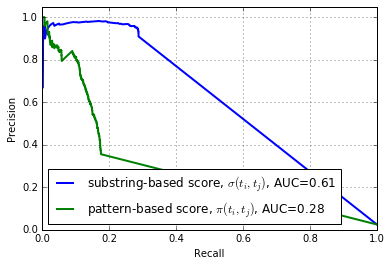
\includegraphics[width=0.5\textwidth]{figures/download}
  \caption{ Precision-Recall plots of substring-based and pattern-based features of the TAXI approach measured on the trial dataset. }
  \label{fig:features}

\end{figure}

\subsection{Candidate Hypernyms via Patterns}
\label{sec:step3}
To extract candidate hypernym relations from texts we used three systems listed below. All of them rely on lexico-syntactic patterns in the fashion of~\cite{hearst1992automatic,klaussner2011lexico}. We used several systems to filter noise via complementary signals. Besides, not all the systems support all the four languages of the SemEval task.  Porting of Hearst patterns to a new European language is a straightforward and relatively quick procedure. Yet, due to a dense SemEval schedule, we decided to implement new rules only for two languages not supported by any available system, namely Italian and Dutch and reuse extraction rules for other languages.  


\textbf{PattaMaika}. This system was used to process English, Italian and Dutch corpora. It implements patterns using UIMA Ruta \cite{kluegl2014uima}. First, part-of-speech information is used to assign  noun phrase (NP) chunk annotations to nominal phrases. Next, we use patterns to identify hypernym relations between NP chunks. % For scalability, we run the pattern extraction on a MapReduce cluster.
We adapted the 9 English rules to the target languages, resulting in 9 patterns for Italian and 8 patterns for Dutch.


\textbf{PatternSim}. This system was used to process English and French corpora. It encodes patterns in the form of finite state transducers implemented with the Unitex corpus processor.\footnote{\url{http://www-igm.univ-mlv.fr/~unitex}} PatternSim relies on 10 English patterns yielding average precision of top 5 extracted semantic relations per word of 0.69~\cite{panchenko12p}. For French, 9 hypernym extraction patterns are used providing precision at top 5 of 0.63~\cite{panchenko2013recherche}.  


\textbf{WebISA}. In addition to \textit{PattaMaika} and \textit{PatternSim}, we used a publicly available database of English hypernym relations extracted from the CommonCrawl corpus~\cite{webisa2016}. We used 108 million hypernym relations with frequency above one. This collection of relations was harvested using a regexp-based implementation of 59 patterns collected from the literature. %The Stanford POS tagger is used for noun phrase identification~\cite{toutanova2003feature}. 


\textbf{Combination of hypernyms}. Result of the extraction are 18 collections of hypernym relations listed in Table~\ref{tbl:hypernyms}. Even the huge \textit{WebISA} collection extracted from tens of terabytes of text does not provide hypernyms for all rare taxonomic terms, such as ``ground and whole bean coffee'' and ``black sesame rice cake''. On the other hand, most of the collections contain many noisy relations.  For instance, frequent relations for hypernyms often go in both directions, e.g. ``history'' is a ``science'', but also ``science'' is a ``history''. Therefore, we introduced an asymmetric pattern-based hypernymy score $\pi(t_i, t_j)$ between terms $t_i$ and $t_j$. It combines information from different hypernym collections to filter noisy extractions. To compute the score, first we normalize extraction counts on the per word basis: $
\pi^k(t_i, t_j) = \frac{freq^k(t_i,t_j)}{\max_j freq^k(t_i,t_j)}
$, where $freq^k(t_i,t_j)$ is the number of relations extracted between terms $t_i$ and $t_j$ by the $k$-th extractor. These normalized scores are averaged across all extractors per language-domain pair:  $
\bar{\pi}(t_i, t_j) = \frac{1}{|LD|} \sum_{k \in LD} \pi^k(t_i, t_j)
$, where $LD$ is a set of hypernym collections relevant for a given language-domain pair. For instance, for the language-domain pair "English-Food", the $LD$ contains four collections: general relations extracted by \textit{PatternSim}, \textit{PattaMaika} and \textit{WebISA} plus domain-specific relations extracted by \textit{PatternSim} (see Table~\ref{tbl:hypernyms}). Finally, to get the pattern-based score, we subtract averaged scores of two terms in both directions: $\pi(t_i, t_j) = \bar{\pi}(t_i, t_j) - \bar{\pi}(t_j, t_i).$ This way, we downrank symmetrical relations like synonyms and co-hyponyms. 

\begin{table}[]
\footnotesize
\centering
\begin{tabular}{l|llll}
            & \textbf{EN}    \ddag, \textdagger,$\S$            & \textbf{FR}\ddag  & \textbf{NL}\textdagger   & \textbf{IT}\textdagger   \\ \hline
General     & 27.6\ddag, 4.9\textdagger, 118.9\S & 3.2  & 2.22 & 0.13 \\
Food        & 24.1\ddag              & 3.8 & 0.47 & 0.05 \\
Environment & 26.3\ddag              & 4.5 & 0.32 & 0.95 \\
Science     & 9.3\ddag               & 2.7 & 0.97 & 0.05
\end{tabular}
\caption{Number of hypernyms in millions of relations. Systems used to extract respective hypernym collections are denoted with \ddag for \textit{PatternSim}, \textdagger for \textit{PattaMaika} and $\S$ for \textit{WebISA}. }
\label{tbl:hypernyms}

\end{table}

The precision-recall curve of the pattern-based score on the trial data is presented in Figure~\ref{fig:features}. This plot is calculated on general corpora as we did not crawl domain specific corpora for the trial dataset domains. As one can see, precision of 0.80 is achieved at recall of 0.15 or less and drops to 0.36 at recall of 0.19. AUC of 0.28 of is less than half of the substring-based score of 0.61. Thus, patterns are  a less reliable source of hypernyms than the substrings. Yet, they can capture relations between words with different spelling like ``apple'' and ``fruit'', while the substring-based score need a character overlap, like in ``grapefruit'' and ``fruit''.   

\subsection{Pruning of Hypernyms}
\label{sec:step4}
Patterns and substrings together yield up to several hundreds of hypernym candidates per term. This step prunes hypernym candidates, ranking them with an unsupervised and supervised combinations of the $\sigma(t_i,t_j)$ and $\pi(t_i,t_j)$ scores. 

\textbf{Unsupervised Pruning}. In this pruning strategy, used for French, Dutch and Italian languages, a term $t_i$ is a hypernym of term $t_j$ if their substring score $\sigma(t_i,t_j)$ is greater than zero or if rank of the term $t_i$ according to the pattern-based score $\pi(t_i,t_j)$ equals to one or two. Thus a term $t_i$ obtains all hypernyms extracted by substrings and up to two hypernyms extracted by patterns.   

\textbf{Supervised Pruning}. This pruning strategy used for English relies on a supervised classifier trained on the trial  dataset~\cite{task13semeval2016}.~\footnote{We did not submit to SemEval both supervised and unsupervised versions of the system for English as only one run was allowed per language-domain pair.} This pruning approach uses 3,249 hypernymy relations from the trial taxonomies as positive training samples, e.g. hypernym relation  (``biology'', ``science'') and 128,183 automatically generated relations as negatives samples coming from two sources:  3,249 inverted hypernyms, such as (``science'', ``biology'') plus 124,934 co-hyponyms from the trial taxonomy, for instance (``biology'', ``mathematics''). 

The classifier used in the competition had two features that characterize a word pair $(t_i,t_j)$, namely substring-, and pattern-based scores $\sigma(t_i,t_j)$ and $\pi(t_i,t_j)$. Note, that the same features were used in the unsupervised approach. We applied an SVM classifier with RBF kernel~\cite{vert2004primer}, tuning kernel meta-parameters within an internal loop cross-validation procedure.  


We tested multiple alternative configurations with extra features, including term frequency, out/in degree of terms in the hypernym graph, term length, expansions of hypernyms based on term clustering and shortest paths in the graph of candidate hypernyms as well as other classifiers including Logistic Regression, Gradient Boosted Trees, and Random Forest. However, none of the above mentioned configurations yielded consistently better results on the trial data than the two feature-based SVM.

To identify hypernyms among a  set of terms $T$, we classify using a model trained on the trial data all possible word pairs except identical ones:  $\{(t_i, t_j): i \neq j; (t_i, t_j) \in T \times T \}$. The pairs classified using the positive class are added to the taxonomy.  

\subsection{Taxonomy Construction}
At this point of the taxonomy construction, we obtained a noisy graph, which may contain cycles and  disconnected components. To remove cycles and to obtain a directed acyclic graph taxonomy we used the unsupervised graph pruning approach of Faralli et al.~\shortcite{Farallietal:15}, which searches for a cycle $C$ using topological sorting of Tarjan~\shortcite{Tarjan:72} and then removes a random edge of $C$ until no cycles are detected in the graph. 

Besides, to improve connectivity of the taxonomy we connect all the nodes of each disconnected component with zero out degree to the taxonomy root. 


\begin{table*}[h]
\footnotesize
\centering
\begin{tabular}{l|lll|lll}
                                  & \multicolumn{3}{l}{ \bf Monolingual (EN)} & \multicolumn{3}{l}{ \bf Multilingual (NL, FR, IT)} \\ \hline
\textbf{Measure}                           & \textbf{ Baseline}    & \textbf{BestComp}    & \bf TAXI     & \bf Baseline      &  \bf BestComp & \bf TAXI       \\ \hline 
Cyclicity                         & \it 0           & \bf 0           & \bf 0        &\it  0             & \bf 0             & \bf 0          \\
Structure (F\&M)                  & \it 0.005      & \bf 0.406      & 0.291   & \it 0.009    & 0.016    & \bf 0.189     \\
Categorisation (i.i.)             & \it 77.67       & \bf 377.00         & 104.50    &\it  64.28         & \bf 178.22        & 64.94      \\
Connectivity (c.c.)               & \it 36.83       & 44.75       & \bf 1  .00      & \it 40.50          & 34.89         & \bf 1.00          \\
Gold standard comparison (Fscore) & \it 0.330        & 0.260        & \bf 0.320     & \it 0.009        & 0.016        & \bf 0.189     \\
Manual Evaluation (Precision)     & \it n.a.        & \bf 0.490    & 0.200     & \it n.a.          & 0.298        &\bf 0.625    
\end{tabular}

\caption{Overall scores obtained by averaging the results over domains (Environment, Science, Food) and languages (NL, FR, IT) for the multilingual setting. The  \textit{BestComp} lists the respective best scores across  four our competitors. The best scores excluding the baseline are set in boldface. Definitions of the measures are available in Section~\ref{sec:evaluation}. }
\label{tbl:results}
\end{table*}



\section{Evaluation}
\label{sec:evaluation}

To assess quality of the taxonomies several complementary  measures were used. The first type of measurements are structural measures, such as the number of connected components (c.c.), the number of intermediate nodes (i.i.), i.e. the number of nodes with out degree equal to zero, and the presence of cycles. Second, system outputs were  compared against the corresponding domain gold standards and performances are evaluated in terms of F-score. Here precision and recall are  based on the number of edges in common with the gold standard taxonomy over the number of system edges and over the number of gold standard edges respectively. To better compare against gold standard taxonomies the task included the evaluation of a cumulative measure \cite{velardi2013ontolearn}, namely Cumulative Fowlkes \& Mallows Measure (F\&M), where the similarity between the system and the reference taxonomies are measured as the combination of the hierarchical cluster similarities. Finally, the organizers performed manual quality assessment to estimate the precision of the hypernyms. To compute this measure, annotators labeled a sample of 100 hypernym relations as correct or wrong. The taxonomy extraction was evaluated on four languages, namely English, Dutch, French and Italian, and three different domains (Food, Science and Environment). A detailed description of the evaluation settings and metrics can be found in \cite{task13semeval2016}.

\section{Results}

Table~\ref{tbl:results} presents a summary of evaluation of our method on the SemEval 2016 Task 13 dataset. Overall 5 systems participated in the challenge: JUNLP, TAXI, NUIG-UNLP, USAAR and QASITT. We represent the respective best scores across our four competitors in the \textit{BestComp} column.
 
\textbf{Gold Standard Comparison.} The organizer-provided \textit{Baseline} system implemented a string inclusion approach that covers relations between compound terms. A similar mechanism was used by the USAAR system~\cite{usaarsemeval2016}, which improved over the baseline in terms of precision at the cost of recall. USAAR achieved the highest precision scores for English, as they used substring-based methods that yield high precision (c.f. Figure~\ref{fig:features}). Yet substrings cannot retrieve hypernyms of non-compound terms.
 
The main mechanisms we added in TAXI with regard to the substring-based methods are statistics over pattern-based extractions over large domain specific corpora and our taxonomy construction step that improves structure of the resource. These united mechanisms are not used in other submissions to the challenge. The NUIG-UNLP team~\cite{nuigsemeval2016} relies on vector directionality in dense word embedding spaces. Such approximation of patterns based on distributional similarity provided good recall, but  attained low precision. 

The QASSIT team~\cite{qassitsemeval2016}, who ranked second in the competition, uses patterns to extract hypernym candidates, but they rely solely on the Wikipedia. Subsequently, an optimization technique based on genetic algorithms is used to learn the parametrization of a so-called pretopological space, which leads to desired structural properties of the resulting taxonomy.  While we use simpler optimization procedure based on supervised learning, TAXI  outperforms QASSIT in terms of comparisons with the gold standard. Possible reasons why our method performs better are (1) QASSIT use no substring features, (2) this team relies on smaller general-purpose corpora, while we use larger domain-specific corpora. 

Finally, JUNLP relies on substrings and relations extracted from BabelNet. We find the latter to be undesirable for taxonomy extraction. Indeed, a rich lexical resource, such as BabelNet can be considered as a taxonomy in itself.  Interestingly, even with the BabelNet-based features the system did not always reach the top precision and recall. 
% We argue that lexical resources of this kind shall be used for evaluation and possible light supervision of an extraction method, but not for feature extraction.

\textbf{Manual Evaluation. } Our system was ranked first in terms of manual judgments for the Dutch, Italan and French reaching the average precision across languages and domains of 0.625. Precision for different language-domain pairs ranged from 0.90 for the Italian-Science pair to 0.23 for the French-Environment pair. For English, our system was ranked second with the average score of 0.20, while the substring-based USAAR system obtained the score of 0.49 and the third-ranked system obtained the score of 0.09. We attribute lower precision in the English run to absence  in the supervised ranking scheme of a limit on the number of extracted hypernyms per word. 

Further detailed comparisons with other systems with breakdowns with regard to different languages, domains and evaluation schemes are presented by Bordea et al.~\shortcite{task13semeval2016} and on SemEval website.\footnote{\url{http://alt.qcri.org/semeval2016/task13}} 

\textbf{Discussion}. One shortcoming of our method is its coverage: for instance 774 terms of 1,555 of the English food domain are still not attached to any node, which is a typical issue with pattern-based approaches since not all taxonomic relationships are spelled out explicitly in corpora. To tackle this shortcoming, we plan to use hypernym expansion  based on distributional semantics \cite{biemann2013text}.

\section{Conclusion}

We presented a technique for taxonomy induction from a domain vocabulary. It extracts hypernyms from substrings and large domain-specific corpora bootstrapped from the input vocabulary. Multiple evaluations based on the SemEval taxonomy extraction datasets of four languages and three domains show state-of-the-art performance of our approach. An implementation of our method featuring all language resources, is available for download.\footnote{ \url{http://tudarmstadt-lt.github.io/taxi}}


\section*{Acknowledgments}

We acknowledge the support of the Deutsche For\-schungs\-gemeinschaft under the JOIN-T project.  



\bibliography{naaclhlt2016}
\bibliographystyle{naaclhlt2016}


\end{document}
